% LLNCS macro package for Springer Computer Science proceedings;
% This is samplepaper.tex, a sample chapter demonstrating the
% Version 2.20 of 2017/10/04
%
\documentclass[runningheads]{llncs}
%
\usepackage{graphicx}
\usepackage{amsmath}
\usepackage{url}

% Used for displaying a sample figure. If possible, figure files should
% be included in EPS format.
%
% If you use the hyperref package, please uncomment the following line
% to display URLs in blue roman font according to Springer's eBook style:
% \renewcommand\UrlFont{\color{blue}\rmfamily}

\begin{document}
%
\title{Real-time Power Prediction in Tour de France}

%
%\titlerunning{Abbreviated paper title}
% If the paper title is too long for the running head, you can set
% an abbreviated paper title here
%
\author{
Yasuyuki Kataoka\inst{1} \and Peter Gray\inst{2}}
%
\authorrunning{Y. Kataoka et al.}
% First names are abbreviated in the running head.
% If there are more than two authors, 'et al.' is used.
%
\institute{NTT Innovation Institute Inc., East Palo Alto CA 94089, USA
\email{kataoka.yasuyuki@ntti3.com}\\
\and
Dimension Data Australia, Port Melbourne, VIC, 3207, Australia\\
\email{peter.gray@dimensiondata.com}}
%
\maketitle              % typeset the header of the contribution
%
\begin{abstract}
This paper introduces the real-time machine learning system to predict power usage of professional riders at {\it{Tour de France}}. In cycling races, it is crucial not only for athletes to understand their power output, but for cycling fans to desire to enjoy this data too. For example, how much riders tactically save energy, which group uses more power, etc. Revealing these insights helps to entertain fans more. However, it is difficult to obtain the power information from each rider directly. Although most teams attach power meters on their bikes, the performance information is usually confidential within the team.  In cooperation with one of the professional teams in cycling sports and Dimension Data's data analytics platform which collects GPS data from all riders, we deployed a machine learning module that predicts power
using the GPS data. 
This paper discusses 1. feature design method and 2. real-time machine learning model analysis. First, the proposed feature design method leverages both hand-made feature engineering using physics knowledge and automatic feature generation using autoencoder. Second, the various machine learning models are compared and analyzed with the latency constraints.  As a result, our proposed method reduced prediction error by 56.79\% compared to the conventional physics model and satisfied the latency requirement so that the system can predict the power of 198 riders per one second. Our module was used during the {\it{Tour de France 2017}} in a real-time manner to indicate {\it{an effort index}} that was shared with fans via media.

%The abstract should briefly summarize the contents of the paper in
%15--250 words.

\keywords{Machine Learning, Recurrent Neural Network, Autoencoder,
Real-time System, Spatiotemporal Data}

\end{abstract}
%
%
%
\section{Introduction}
%筋疲労を理解することは、多くのスポーツにおいて極めて大きなインパクトを持つ。
%例えば、自転車競技やアイススケート(short track, mass start or pursuit)など、相手との駆け引きが重要となる競技においては、筋力をsave、或いはburstさせるタイミングを適切に判断することが勝利への鍵となる。
%こうした筋力のマネージメントは、プロフェッショナルな競技においては、選手チームと観客にとって特に重要である。
%選手チームの観点では、相手の戦略やパフォーマンス(capability)を知ることで、相手の裏をつく戦略を立てることが可能になる。
%観客の観点では、選手の筋疲労をリアルタイムに知ることができれば、スポーツをより深く楽しむ事が可能となる。
%しかしながら、筋疲労のデータは通常、機密情報となっており、簡単に取得できるものではない。
%こうした背景から、本論文では筋疲労データを予測するツールを提案すること、を目的とする。

% スポーツ全般に言える筋力の重要性
Understanding muscle fatigue has a significant effect on many sports. It is the key for victory to judge the timing to save or exert muscular strength particularly in Cycling and Speed skate(Short track, Mass start, Pursuit). Such muscle management is crucial for athletes and audiences in professional competitions. For athletes, knowing the performance of the opponent makes it possible to strategize their tactics against the other party's one proactively. For audiences, knowing the player's muscle fatigue in real time allows them to enjoy the sports more deeply.

% 自転車競技における筋力の重要性
Among many sports, this paper focuses on cycling. Measurement of muscle power in cycling has become an attractive tool for professional riders, coaches, and amateurs to improve the riding performance. For instance, it allows coaches to help monitor the effectiveness of training and set accurate training programs when combined with heart rate measurement. It also allows riders to tactically determine energy use by analyzing other's muscle fatigue level. Moreover, it helps audiences to predict whether Peloton, the main group of the race, will catch the front of the race.

% 筋力を把握における課題
However, there are two issues in power data collection in cycling sports. First, power sensors tend to be expensive. Reducing cost of power meters means that they are becoming more accessible to competitive and even recreational amateur cyclists. As a result, there is increasing interest in understanding the power output of the professional cyclists. Second, data on muscle usage is usually highly confidential, and it is not easily accessible. It is difficult to directly obtain the power data from professional riders due to its competitive sensitivity. Although most professional teams attach power meters, the performance information is usually confidential within the team.

% この論文の目的
The purpose of this paper is to create the real-time muscle power prediction tool for cycling sports to enable people to get access to power data. This applied data science paper discusses the design process of our real-time machine learning system that predicts the power usage of professional riders at {\it{Tour de France}}\footnote{{\it{Tour de France}} is one of the
three major European professional cycling stage races in road bicycle
racing.  \url{https://en.wikipedia.org/wiki/Tour_de_France} }.

% 先行手法の問題点
Conventionally, the power data is analyzed by the physics model which heavily relies on not data-driven but model-driven approach. This approach heavily depends on the physical constants, which tends to be less accurate. The challenge of the data-driven approach is collecting the labeled data with power information along with GPS data. Fortunately, in cooperation with one of the professional cycling teams and {\it{Dimension Data's data analytics platform}} \footnote{Dimension Data's data analytics platform,
\url{https://www2.dimensiondata.com/tourdefrance/analytics-in-action}} which collects GPS data from all riders, we obtained the labeled dataset for this purpose.

% この論文の貢献・技術的内容
This paper, in general, discusses the data-driven approach that also fuses the physics knowledge with the focus on 1. feature design method and 2. real-time machine learning model analysis. First, the proposed feature design method leverages both hand-made feature engineering using physics knowledge and automatic feature generation using autoencoder. Beyond the previous studies of muscle fatigue analytics for cyclists, the feature inspired by deep learning enables trajectory patterns to be embedded to Machine Learning model. This generated feature allows us to implicitly consider the rider's behavior such that the power use is loosened in the context of turning a sharp corner on a downhill slope. Second, the various machine learning models are analyzed under the latency constraints. The tree-based model and time-series deep learning models are compared regarding latency and error rate.

% 結果
As a result, our ultimate model reduced prediction error by 56.79\% compared to the conventional model-based model that depends on the prior knowledge of physics. Our Machine Learning module was used during the {\it{Tour de France 2017}} in a real-time manner to create {\it{an effort index}} that was shared with fans via social media. Our proposed method can be used for amateur riders too who want to know the power performance but does not want to purchase a real power meter which tends to be very expensive.

\section{Related Work}
The performance of cycling riders has been studied across various
academic fields.\cite{ref_1} Among them, this paper focuses on muscle fatigue and
addresses the problem of predicting it by machine learning. This section
shows articles on muscle fatigue and machine learning application using
cycling data.


\subsection{Fatigue Analytics}
In the study of muscle fatigue in cycling, models considering various
factors have been proposed. For example, one proposed model considers
physiological, biomechanical, environmental, mechanical and
psychological factors and integrates them into nonlinear complex system
models.\cite{ref_2} While many researchers take the model-based
approach\cite{ref_3}\cite{ref_4}, this paper focuses on a data-driven
approach using the limited available dataset such as GPS.

The fatigue analytics is, in general, used for performance or safety
improvement in the sports industry. One example is finding the
relaxation place during a race.\cite{ref_5} Contrary to the past
studies, our ultimate aim of this paper is mainly for fan engagement,
which is also important in sports industry from the business
perspective.

\subsection{Machine Learning Application using cycling data}
The most famous machine learning applications using cycling GPS data is
the transportation mode prediction: classifying user's activity to
bicycle, car, train, walk, run and others.\cite{ref_6} One study
reported that the generated feature from GPS trajectory using Deep
Learning improves accuracy.\cite{ref_7} This is because the Deep Learning
automatically captures important features which are difficult to be
designed explicitly by hand-made feature engineering.\cite{ref_8}

In our limited but best knowledge, there is no research report about
muscle fatigue prediction using both hand-made feature and generated
feature by deep learning. Moreover, this paper also reports the
comparison between model-drive and data-driven approaches for muscle
power prediction in cycling sports.

\section{Dataset}
This section describes the input data and the labeled data obtained by sensors.

\subsection{Input Data: GPS and wind sensor} \label{sec:input_data}
{\it{Dimension Data's data analytics platform}} has a live GPS tracking system. This system provides the GPS tracking of position and speed for all riders at a 1-second frequency from the GPS sensors mounted under the bicycle saddle. This data is processed in real time, and enriched to calculate key metrics such as distance to finish, position in the race, time gaps, clustering of individual riders into groups, and the additional data such as the current gradient of the road at that point, as well as the wind conditions at that location.

The detail of the backend system to collect these real-time data is described in Appendix A.

\begin{figure}[t]
 \begin{center}
  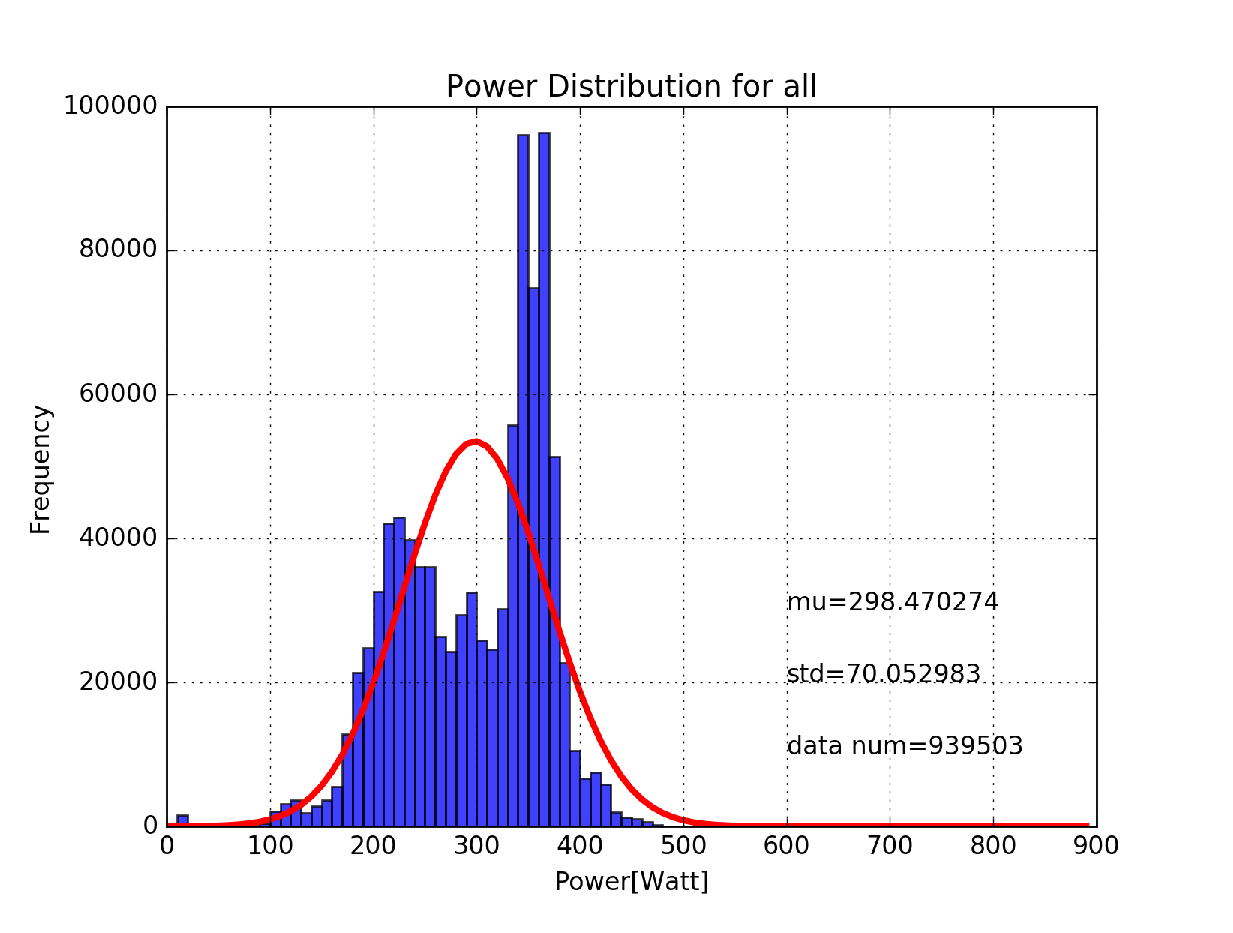
\includegraphics[width=0.8\textwidth]{fig/dist_bib_all.eps}
  \caption{Power Distribution: The imbalanced data makes hard to predict the high or low power range}
  \label{fig:power_distribution}
 \end{center}
\end{figure}

\subsection{Labeled Data: Power sensor}
Power is the measurement of how much force is being pushed through the pedals by the rider and is measured using dedicated sensors usually built into cranks, pedals or rear wheel hub. Most power meters connect wirelessly to the rider's bike computer allowing them to monitor their power output during a training session or race and manage their effort accordingly.

In this project, a training dataset was obtained from one of the professional cycling teams in previous professional races. This dataset includes the data {\it{Dimension Data's data analytics platform}} provides as well as the power sensor data in accordance with the time stamp. The distribution of the power data is shown in Fig. \ref{fig:power_distribution}. Since this dataset is rare for the machine learning project, this research project could be the first study on power prediction based on the GPS data of professional cyclists in our best knowledge.

\section{Methodology}
This section mainly describes how the machine learning model is designed for power prediction with the focus on 1. feature design method and 2. real-time machine learning model analysis. 

In the feature engineering part, the hand-made feature is designed by mechanical factors using fundamental physics. Also, the generated feature by autoencoder is concatenated to the feature space.

In the regression model, the various machine learning models are introduced with the arguments of advantages and latency perspectives.

\subsection{Feature Engineering}
Our proposed feature design is shown in
Fig.\ref{fig:machine_learning_pipeline}: a hand-made feature inspired by
physics knowledge and an automatically generated feature using deep
learning.

\begin{figure}[t]
 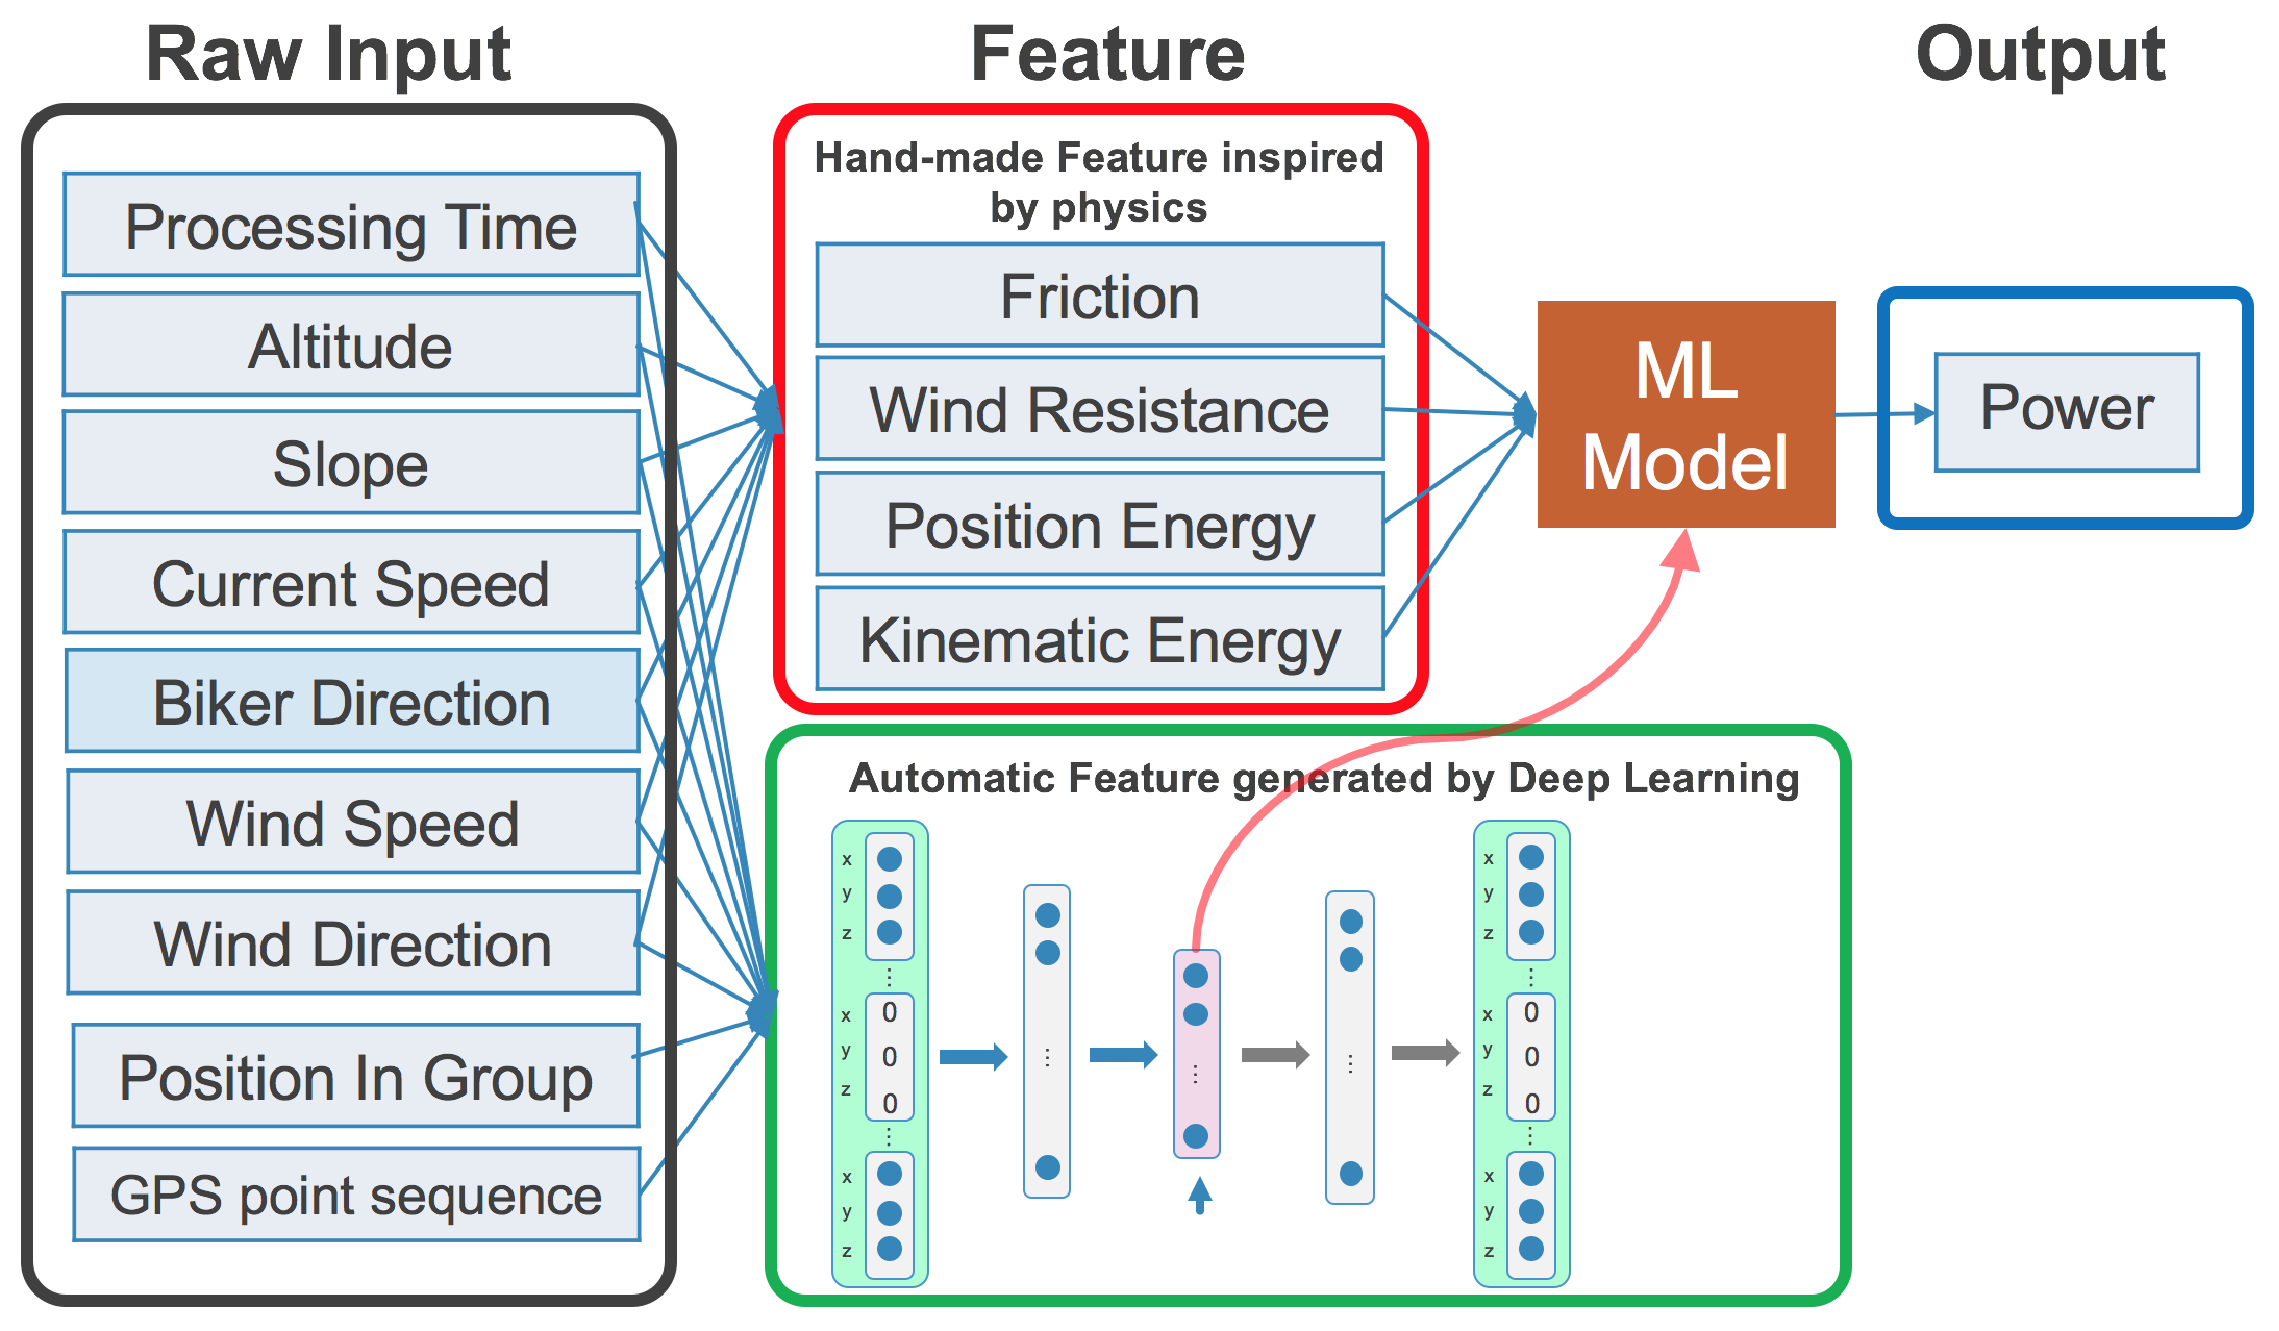
\includegraphics[width=\textwidth]{fig/machineLearningModel.eps}
 \caption{Machine Learning pipeline: Raw input is obtained from
 {\it{Dimension Data's data analytics platform}}. Both hand-made feature
 by physics and automatic feature generated by Deep Learning is
 concatenated for Machine Learning model.}
 \label{fig:machine_learning_pipeline}
\end{figure}

\subsubsection{Hand-made Feature} \label{sec:hand_made_feature}
Physically, the power of the rider is determined by four factors: 
\begin{enumerate}
 \item “friction with the ground” denoted as $P_f=C_f v_b mg$, where $C_f$
       is the friction coefficient, $v_b$ is the velocity of a bicycle, $m$
       is the mass of a rider and a bicycle, and $g$ is standard gravity.
 \item “wind resistance” denoted as $P_w= 1/2 C_d A \rho(v_b-v_w )^2$,
       where $C_d$ is drag coefficient, $A$ is frontal cross-section area,
       $\rho$ is air density, and $v_w$ is wind velocity.
 \item “kinetic energy” denoted as 
       $P_k=\frac{m}{2\Delta T}(v_n^2-v_p^2)$, where $v_n$ is the velocity 
       at $t=now$[sec], and $v_p$ is the previous velocity at $t=now-\Delta T$[sec].
 \item “potential energy” denoted as $P_p = mg\frac{\Delta h}{\Delta T}$, 
       where $\Delta T$ is sampling time interval, and $h$ is height variation 
       within $\Delta T$.
\end{enumerate}
	
For each, theoretical values of these coefficients are
known.\footnote{one example of the physical constants\\ \url{http://socrates.berkeley.edu/~fajans/Teaching/CalcsWeb.htm}}
However, we realized that the power calculated by these theoretical
values is greatly different from the data from real sensors. Therefore,
the power prediction model is designed by machine learning, which
identifies the desired coefficients to fit with real sensor values.

Since it is known that $P_w$ is the most dominant factor to compute
muscle power, the wind data around rider $v_w$ is also considered for
precise wind resistance estimation. Plus, it is worthwhile to remark
that the position in the cluster is also considered as one of the
features because it dramatically affects power use. For example, it is
said that a rider in the second row uses approximately 50\% of the power
that a rider in the first row uses.


\subsubsection{Generated Feature by Deep Learning}
It is assumed that the rider's power use is influenced by past and future trajectory of a rider. For example, it is observed that the pedal is stopped in the context of turning a sharp corner on a downhill slope. Therefore, consideration of trajectory pattern should improve power prediction accuracy. However, we found a problem in applying original GPS trajectory data to learn machine learning model. Since GPS trajectory data tends to be very sparse, there was little impact on the accuracy improvement. There are two reasons for this problem: 1. direction diversity, 2. high dimensionality.

First, normalization of the trajectory direction is performed in the $(x, y)$ plane. As shown in Fig.\ref{fig:data_normalization}, the rotation transformation is applied so that the direction of the vector towards the position after $N\Delta$ seconds corresponds to the positive direction of the $y$-axis. Here, the future GPS points are predicted based on the assumption that the current speed is maintained along with the course track. After applying rotation normalization, standardization is applied for each $x$, $y$, and $z$-axis.

\begin{figure}[t]
 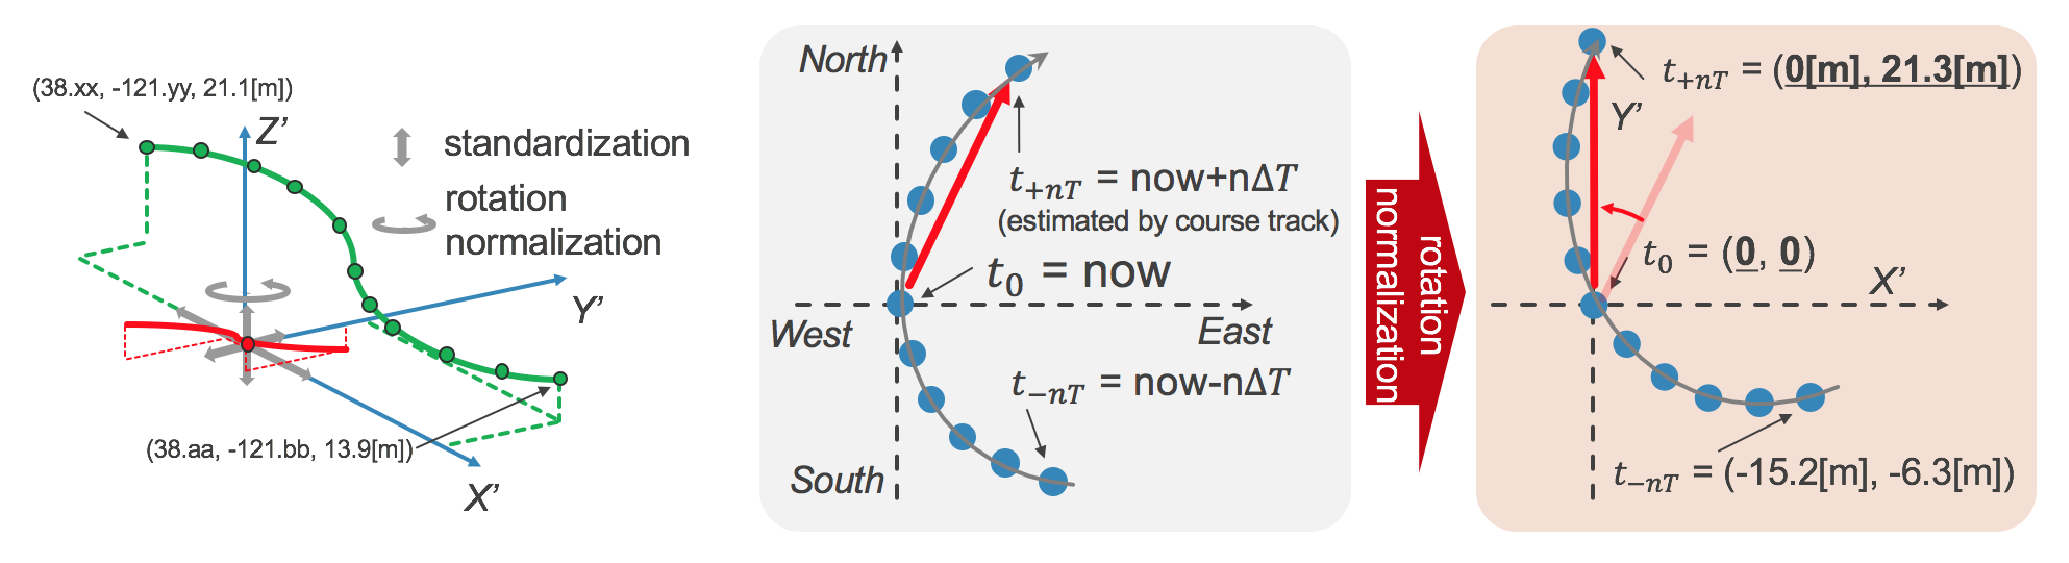
\includegraphics[width=\textwidth]{fig/data_normalization.eps}
 \caption{Data normalization for GPS trajectory}
 \label{fig:data_normalization}
\end{figure}

Second, a dimensional reduction is applied by autoencoder. There are a variety of autoencoders such as denoising autoencoder\cite{ref_9}, deep autoencoder\cite{ref_10}, and stacked deep autoencoder\cite{ref_11}. They are all compared and analyzed when applied to this trajectory embedding problem. The input vector is the GPS points from $t-N\Delta T$ to $t+N\Delta T$, where each GPS point has $x$, $y$, and $z$ value as shown in Fig.\ref{fig:deep_autoencoder}. This ends up a total 3(2$T$+1) dimension for input space. In the deep autoencoder, weights are learned so that the output becomes same as the input with multiple intermediate layers sandwiched therebetween. These deep layers make it accurate to restore the input, meaning that implicit but powerful feature of the trajectory is extracted automatically. In this paper, the compressed feature vector by deep autoencoder is called the 'embedded trajectory feature'. This embedded trajectory feature is concatenated to the hand-made feature. Then, this overall feature can be used as an input to regression models.

\begin{figure}[t]
 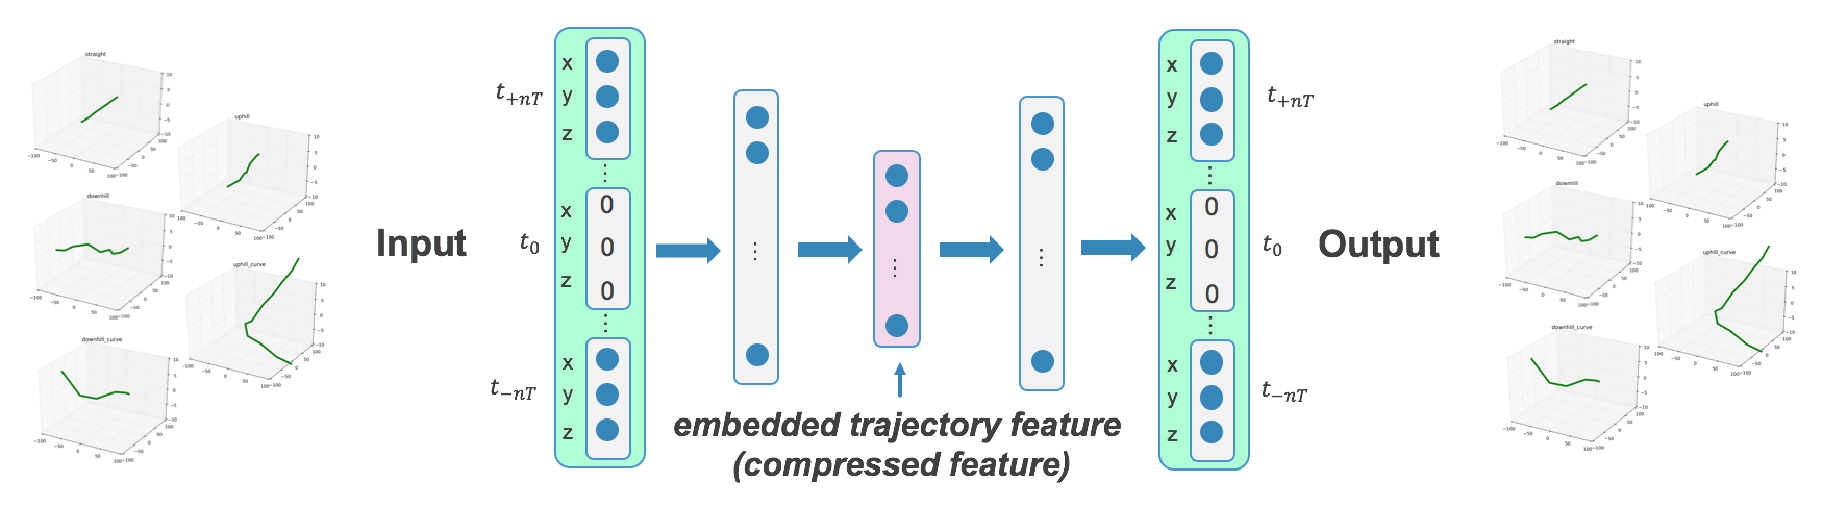
\includegraphics[width=\textwidth]{fig/deep_autoencoder.eps}
 \caption{embedded trajectory feature by autoencoder}
 \label{fig:deep_autoencoder}
\end{figure}

%\subsection{Kalman Filter}
%Our system is expected to sample GPS data every second, but occasionally
%network connectivity or sensor issues result in data gaps or errors. To
%mitigate these impacts, Kalman Filter is applied.[10] In our system, the
%machine learning prediction is used for ‘measurement', and dynamical
%system prediction is used for 'estimation'. The dynamical system is
%designed to be a linear model such that 
%\begin{equation}
%\frac{d}{dt}x = 
% \begin{bmatrix}
%  1 & \Delta t \\
%  0 & 1
% \end{bmatrix}
% x
%\end{equation}
%, where $x = [\tilde{p}, \tilde{\dot{p}}]$, $\tilde{p}$ is the power
%predicted and ∆t is the time duration since the last sampling.

\subsection{Regression Model} \label{sec:regression_model}
Several regression models are tested with the aim of the real-time scenario. The challenge of the model choice is, in general, to find the best model regarding latency and error rate.

In our real-time power prediction application, the latency is a critical issue. Our system must predict power for each of 198 riders within one second. In the case of simple scenario by one machine, it is necessary to complete one prediction approximately at 5 msec. Within this 5 msec, the following process needs to be completed: extract dataset from the database, run feature engineering, run inference, and send prediction outcome to the database. Although the distributed computing can solve this latency issue in the real scenario by the parallel computation, we consider the latency requirement 2.0[msec] in consideration of the limited project budget.

\subsubsection{Tree-based Models}
Random Forest\cite{ref_12} and XGBoost\cite{ref_13} are considered as part of the regression model candidates. The advantage of the decision tree type model is that the number of trees in the model can easily be adjusted. This parameter afffects the inference latency. Plus, the tree-based models have a chance to outperform the deep learning models when data is not sufficiently adequate. In addition to it, the tree-based model is explanatory to analyze the cause of the muscle fatigue.

The hyperparameters are tuned by grid search through several experiments except for the number of trees.

\subsubsection{Time-series Deep Learning Models(Recurrent Neural Net)}
Stacked Long Short-Term Memory(LSTM)\cite{ref_14} and Gated Recurrent Units(GRU)\cite{ref_15} are considered as part of the regression model candidates from Recurrent Neural Net(RNN) models. The advantage of RNN is that predictive performance may outperform other models by extracting effective features over time-series information.

After several experiments, some hyperparameters are fixed, e.g., the number of the past time-series data = 10, dropout ratio = 0.4. In this paper, the number of the layer numbers is treated as hyperparameter.

\section{Result}
First, this section quantitatively evaluates the accuracy of the power prediction regarding feature engineering, embedded trajectory feature, and regression models. Moreover, this section qualitatively evaluates the impact of the use of this machine learning model on fan engagement at the {\it{Tour de France 2017}}.

In the evaluation, {\it{stratified}} 5-fold cross validation is applied, because the dataset is imbalanced data. The metrics for the evaluation is mean absolute error (MAE), which computes the absolute value between the predicted value and the ground truth.

\subsection{Feature Engineering}
The purpose of this section is to analyze the effect of feature engineering by both hand-made features inspired by physics and generated feature by trajectory embedding autoencoder. In this comparison analysis, the following four different model types are considered:
\begin{enumerate}
 \item M1: Model-Based Model (baseline)

       This is the conventional power model which only relies on only
       fundamental physics. This model is designed by the sum of four
       power factors, $P=P_f+P_w+P_k+P_p$, where coefficients and
       parameters are determined by our best knowledge with literature
       previously cited in this paper.

\item M2: Data-Driven Model without Feature Engineering
      
      This is a data-driven model without any additional feature engineering. This machine learning model simply uses raw input that is obtained from {\it{Dimension Data's data analytics platform}} described in \ref{sec:input_data}. 
      
\item M3: M2 + Hand-made Feature 
      
      In addition to M2, the model M3 considers the hand-made feature designed in \ref{sec:hand_made_feature}.

\item M4: M3 + Embedded Trajectory Feature by denoising stacked autoencoder
      
      In addition to M3, the model M4 considers the embedded trajectory feature designed in section 4.1.2. In this experiment, the parameters are set as $N$=5 and ‘the dimensions of layers' = [33, 20, 10, 20, 33] from input to output. The autoencoder type is chosen to be the denoising stacked autoencoder.
\end{enumerate}

 \begin{table}[t]
  \begin{center}
   \caption{Performance comparison between four different feature engineering by MAE.}
   \label{tab1:MAE_result}
   \begin{tabular}{|c|c|c|c|}
    \hline
    Model Type & MAE (Train) & MAE (Test) & Error Reduction to Baseline\\
    \hline
    M1(Baseline) & - & 139.17 & 0.0\% \\
    M2 & 37.55 & 89.90 & 35.40\% \\
    M3 & 24.36 & 66.82 & 51.99\% \\
    M4 & 21.86 & 60.13 & 56.79\% \\
    \hline
   \end{tabular}
  \end{center}
 \end{table}

 \begin{figure}[t]
  \begin{center}
  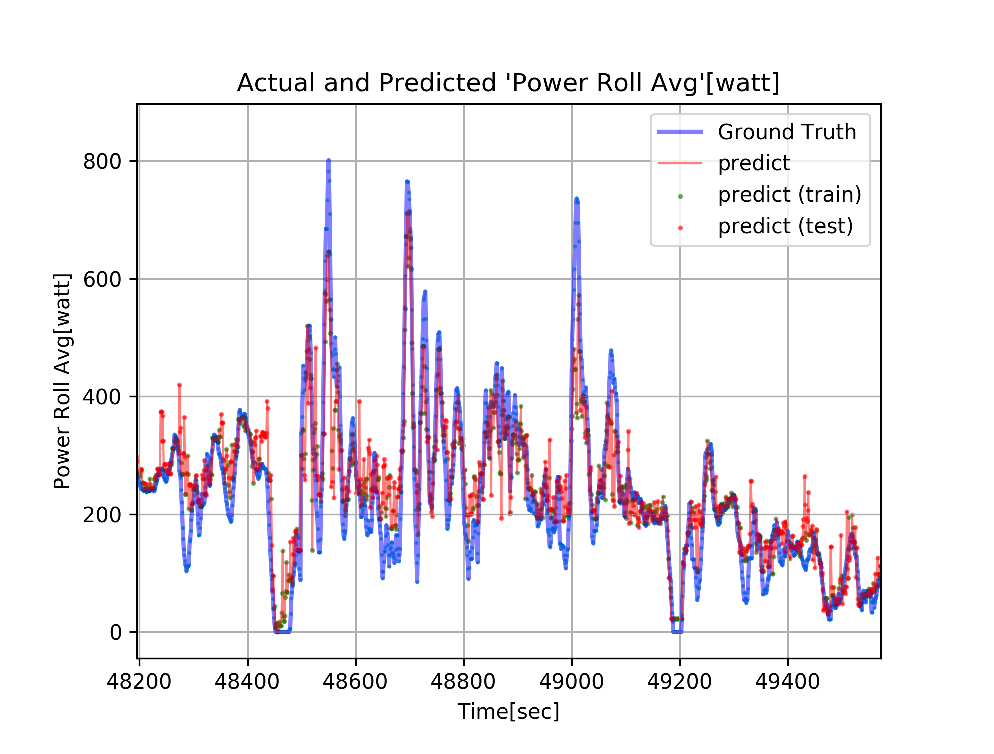
\includegraphics[width=0.8\textwidth]{fig/RF_middlePhysicsPowerRollAvgFixed_graph_7.eps}
  \caption{An example of power prediction with the comparison to ground truth}
  \label{fig:power_prediction_example}
  \end{center}
 \end{figure}

The result is shown in Table. \ref{tab1:MAE_result}. Although the
prediction may be difficult in high power range ($>$400 watt) or low power
range ($<$100 watt) due to the imbalanced training dataset, Fig.
\ref{fig:power_prediction_example} indicates our proposed model can work
accurately in these challenging ranges too.  Then, the comparative
evaluation is shown in Table 1. Our proposed method, M4, outperforms the
simple model-based model using only physics by 56.79\% error reduction in
MAE. Compared to M2, the simple data-driven model, our feature design
improves machine learning model by 35.40\% error reduction in this
experiment. Thus, both hand-made feature and embedded trajectory feature
should help to capture important factors to predict power use in
cycling.



\subsubsection{Analysis of embedded trajectory feature by various autoencoder}
In this section, various autoencoder performances are compared here. In addition to the labeled data of power data, there are a larger amount of the trajectory path data available that is utilized in this experiment. 
On every autoencoder models, the space for the embedded trajectory
feature is constrained to 10 dimensions. The results are summarized in Table. \ref{tab1:autoencoder_result}. First, the Denoising autoencoder improves MAE by 2.2\% compared to the regular autoencoder. Thus, adding denoising effect seems to have the advantage to extract key feature. Next, While the deep autoencoder simply increases the layer, stacked autoencoder train the hidden layer one by one. This ends up improving MAE by 7.46\% compared to the regular autoencoder. Therefore, the denoising Stacked autoencoder is used for the extracting trjectory embbed feature from the GPS sequence data.

 \begin{table}[t]
  \begin{center}
   \caption{Performance comparison between autoencoder Model}
   \label{tab1:autoencoder_result}
   \begin{tabular}{|c|c|c|c|}
    \hline
    Model Type & Parameter & Error Rate to AE\\
    \hline
    autoencoder & [33, 10, 33] & 100.0\% \\
    Denoising autoencoder &  [33, 10, 33] & 97.8\% \\
    Denoising Deep autoencoder & [33, 20, 10, 20, 33] & 96.82\% \\
    Denoising Stacked (Deep) autoencoder & [33, 20, 10, 20, 33] & 92.54\% \\
    \hline
   \end{tabular}
  \end{center}
 \end{table}

\subsection{Regression Model}
The tree-based models and time-series deep learning models are analyzed compared regarding inference latency and error rate.

\begin{figure}[t]
 \begin{center}
  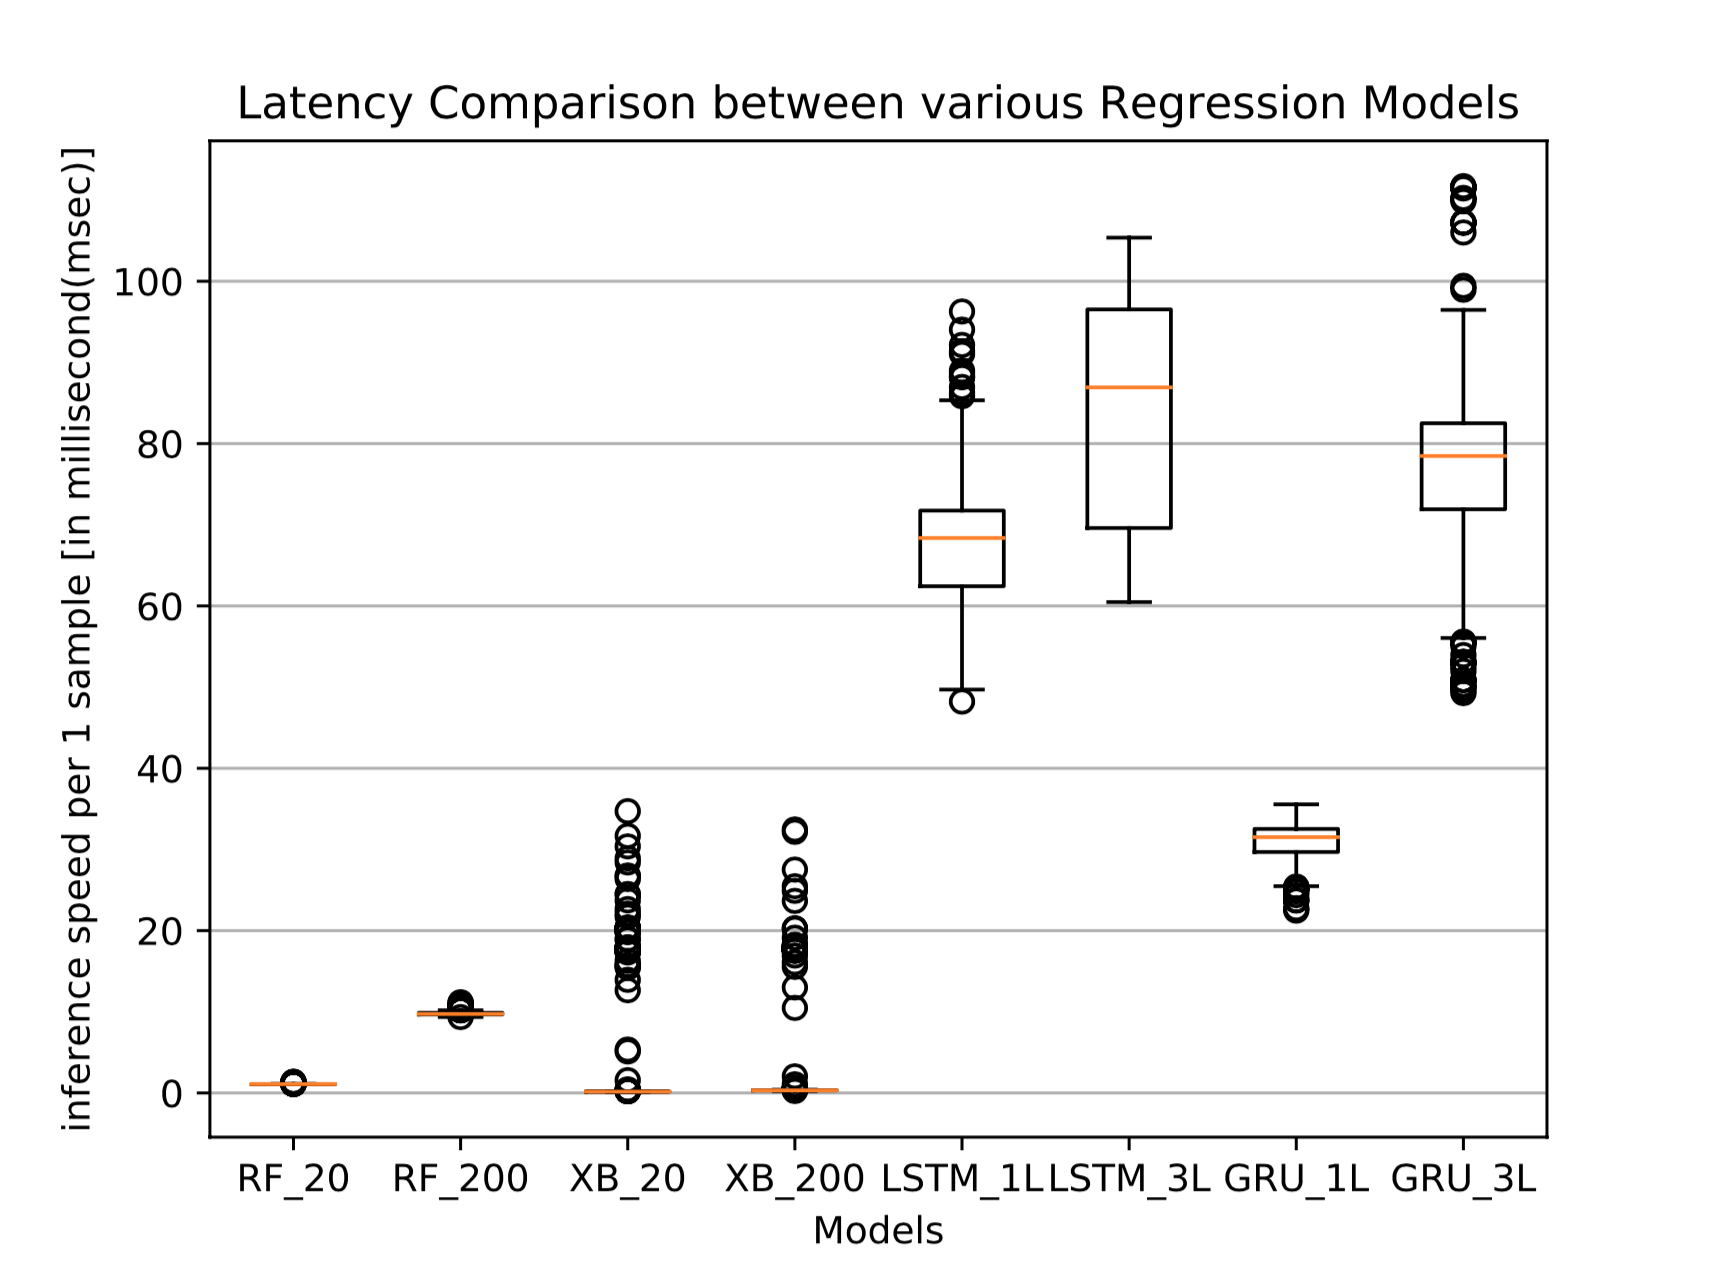
\includegraphics[width=0.8\textwidth]{fig/latency_comparison2.eps}
  \caption{Latency Comparison between different regression models (RF=Random Forest, XB=XGBoost, \_20,\_200= estimation by 20,200 trees, LSTM\_1,\_3=LSTM by 1,3 layers, GRU\_1,\_3=GRU with 1,3 layers)}
  \label{fig:latency_comparison}
 \end{center}
\end{figure}

\subsubsection{Inference Latency}
In this experiment, the inference process was run on 198 samples data on GPU server(Tesla K80) whose status is idle except for this experiment. Note that the computation of 198 samples by matrix must not be run at once, because it needs to be done one by one in the real scenario. The results of the inference latency analysis are shown in Fig. \ref{fig:latency_comparison} by box plot.

The best latency performance measured by median is XGBoost with the 200 trees. While the average performance of XGBoost outperforms other regression models, the latency widely varies and takes +10[msec] for some cases. This anomaly causes the negative impact on the backend system. One negative effect is missing values. The backend system terminates the inference process and then returns NaN for some cases. Contrary to XGBoost, Random Forest fairly performed stably. Random Forest with 20 tree trees satisfies the latency requirement, which is set to be 2[msec] as described in \ref{sec:regression_model}.

The time-series deep learning models, LSTM and GRU does not satisfy our latency requirement. When the multiple layers are stacked, obviously the latency gets worse due to the additional computation.


\subsubsection{Eror Rate - MAE}
In this section, the error rate is argued. The result is shown in Table. \ref{tab1:MAE_latency_result}.

Originally, the time-series deep learning models, LSTM and GRU, were expected to perform much better than this results. In our practical research project, it surely ends up underfitting. One training example is shown in Fig.\ref{fig:stacked_lstm_training}

\begin{figure}[t]
 \begin{center}
  \includegraphics[width=0.7\textwidth]{fig/LSTM_LB5_performance_MAE_Epoch.eps}
  \caption{Stacked LSTM: validation MAE performance over epochs: }
  \label{fig:stacked_lstm_training}
 \end{center}
\end{figure}
One famous way to avoid underfitting is to change the model to deeper structure. Thus, multiple layers such 3, 5, 7 layers were also tested. However, it did not get even close to 100 by MAE. As a conclusion in this project, the more labeled dataset needs to be collected to train the effective model. While it may get outperform tree-based models in future, the latency result indicates another challenge. The latency performance is less stable and takes a longer period for inference on average as shown in Fig. \ref{fig:latency_comparison}.

Among the tree-based models, XGBoost (n\_est=200) has shown the best performance with the satisfactory latency on average. However, it has the problem of the unstable latency issue. Thus, the Random Forest (n\_est.=20) is considered to be the best regression model in our practical situation.

\begin{table}[t]
 \begin{center}
  \caption{Performance Comparison between Regression Models by MAE and latency}
  \label{tab1:MAE_latency_result}
  \begin{tabular}{|c|c|c|c|}
   \hline
   Model Type & MAE (Train) & MAE (Test) & Average Latency[msec]\\
   \hline
   %rf_20
   Random Forest (n\_est.=20) & 24.35 & {\bf{66.81}} & {\bf{1.09}}\\
   %rf_200
   Random Forest (n\_est.=200) & 23.48 & {\bf{66.02}} & 9.76\\
   %xb_20
   XGBoost (n\_est=20) & 32.02 & 70.72 & 2.94\\
   %xb_200
   XGBoost (n\_est=200) & 0.37 & {\bf{63.97}} & {\bf{1.07}}\\
   %lstm_1
   LSTM (1 Layer) & 289.18 & 296.01 & 67.79\\
   %lstm_1
   LSTM (3 Layer) & 280.49 & 289.21 & 84.22\\
   %GRU_1
   GRU (1 Layer) & 289.78 & 290.78 & 30.72\\
   %GRU_3
   GRU (3 Layer) & 280.49 & 289.22 & 77.02\\
   \hline
  \end{tabular}
 \end{center}
 \end{table}

\subsection{Qualitative Analysis}

\subsubsection{Real Deployment in Tour de France 2017}
Our proposed machine learning model was successfully implemented in Dimension Data's data analytics platform. In {\it{Tour de France 2017}}, we converted the power[watt] to {\it{an effort index}} which indicates the power level from 1 to 10 for better visualization to fans and for respects to rider's semi-private data. In the practical data science application that predicts personal data and opens to the public, this process was very important.

As a result, {\it{an effort index}} is successfully predicted for 198 riders every one second in a real-time manner in {\it{Tour de France 2017}}. This was the first trial to deploy the effort index prediction algorithms in the history of {\it{Tour de France}} or any other cycling competition in our best knowledge.
%In the real deployment system, scaling computinng resources had impact
%on some functions described in this paper were tweaked due to some
%constraints in latency requirements and computing resources. 

Fig. \ref{fig:power_comparison_2group} shows one of the real-time visualization tools using the power prediction. This tool enables a user to compare the performance of two different groups at specific time range: e.g., Peloton vs Front Group in the past 5 minutes. This can visualize how enthusiastically peloton saves energy during a race or tries to catch up the front group. In future, this predicted value can be utilized as a significantly important feature in order to predict if the catch happens by Peloton or not. Apparently, the accumulated muscle fatigue is an important feature for this prediction task.

\begin{figure}[t]
 \begin{center}
 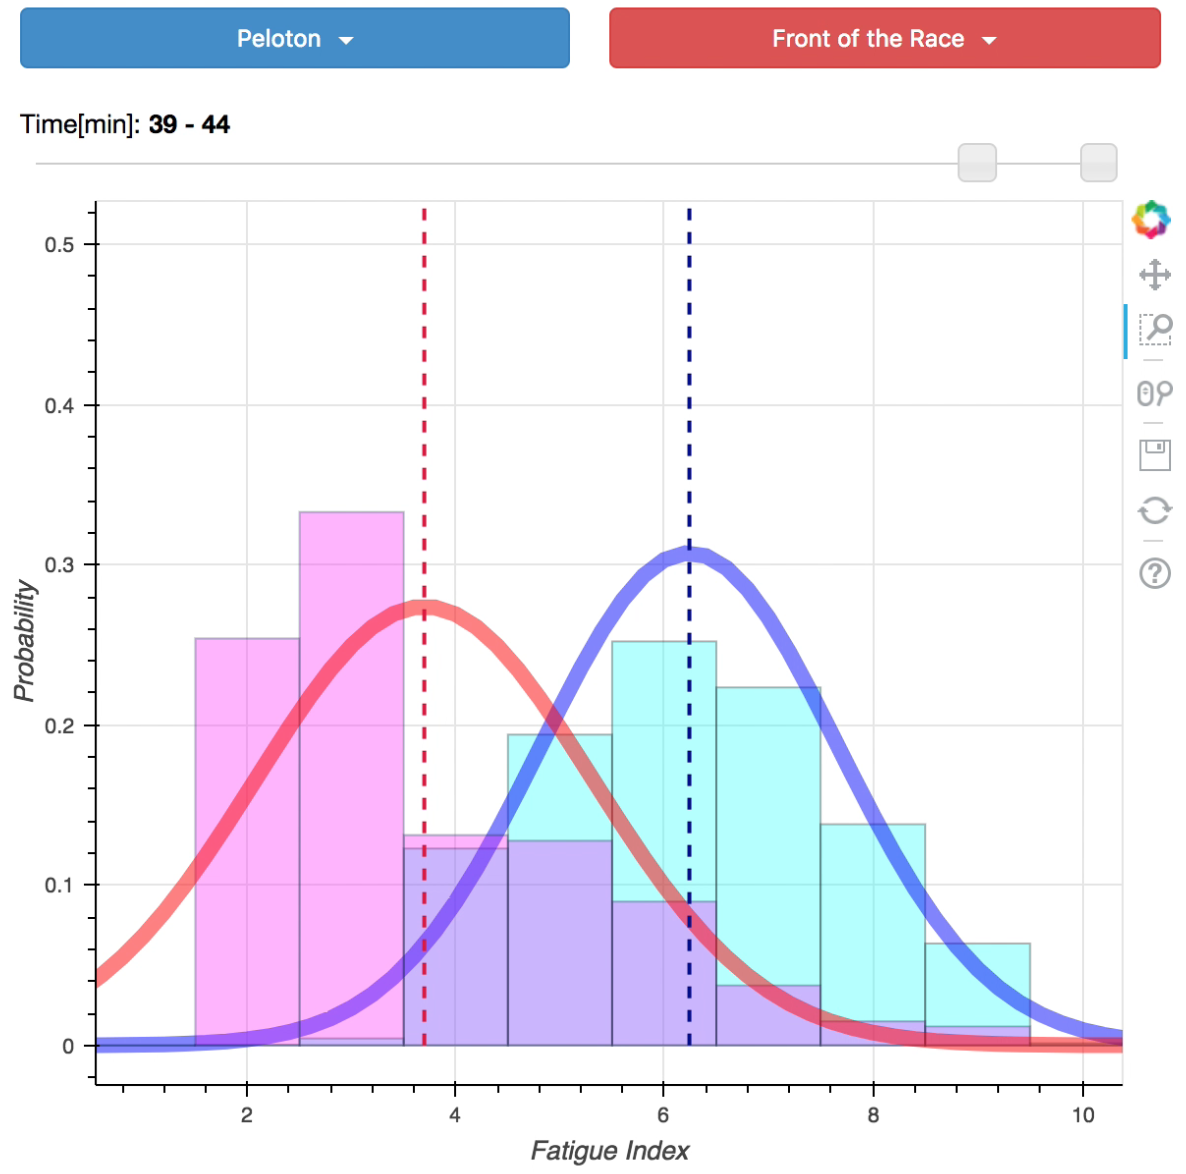
\includegraphics[width=0.7\textwidth]{fig/power_comparison.eps}
 \caption{Power Distribution for two group: x-axis means fatigue index, y-axis means probability, each bar chart means power distribution for two different rider groups.}
 \label{fig:power_comparison_2group}
 \end{center}
\end{figure}

Fig. \ref{fig:power_prediction_graph} shows the social media exposures of our technology: one tweet by Dimension Data that describes how the winner on stage 18 expends energy in accordance with terrain variation of the course. This graph indicates how the winner saved at downhill before the final uphill and used the peak effort at the end of the race.

\begin{figure}[t]
 \begin{center}
 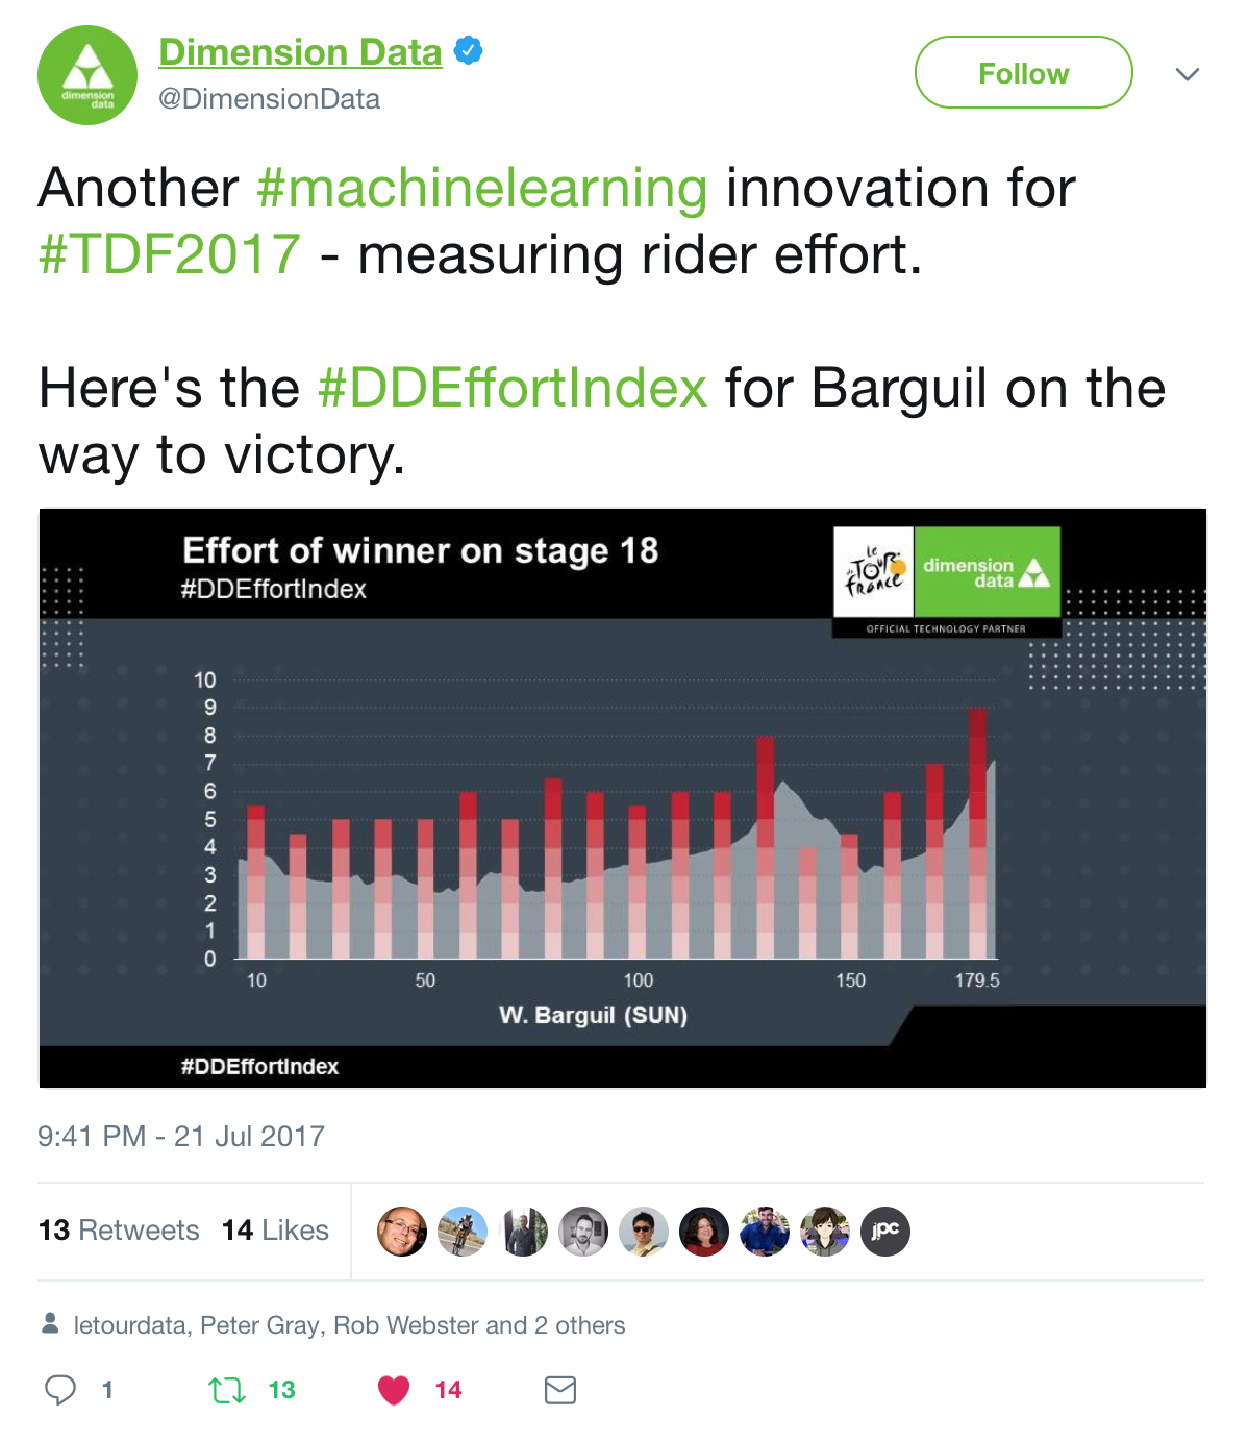
\includegraphics[width=0.6\textwidth]{fig/TDF_tweet_power_prediction2.eps}
 \caption{Example of Social Media Exposure: Visualization of the winner's performance in accordance with the terrain variation}
 \label{fig:power_prediction_graph}
 \end{center}
\end{figure}

\subsubsection{Evaluating the impact on Fan Engagement}
The inclusion of machine learning based insights along with other innovations contributed towards over 20\% year on year growth in social media engagement with fans, with data and insights from this program being referenced regularly across television broadcast, print and digital media, and social media. This is a strong indication of the audience appetite for enhanced data and analytics in professional cycling.

Our proposed methodology and the deployment of it to {\it{Tour de France 2017}} were acknowledged by key business leaders involved in the sport.

{\it{''The introduction of Machine Learning into the live race analytics at the Tour de France has enhanced our ability to create engaging content for fans and commentators, and metrics such as the effort index allow us to better explain the race tactics.''}} – Scott Gibson, Group Executive – Digital Practice, Dimension Data

\section{Conclusion}
This paper presented a machine learning application of power prediction used in {\it{Tour de France 2017}}. The characteristic approach of this paper is the feature design combined with both hand-made feature based on physics and generated features based on denoising stacked autoencoder. Considering the GPS trajectories by Deep Learning, it implicitly considers the factors of rider's intuitive judgment such as the tendency to loosen the force in the curve of the descending slope. As a result, the error (MAE) rate is reduced by 56.79\% compared to the physical model, and by 21.39\% compared to the basic machine learning model. Moreover, several regression models are investigated regarding error rate and latency. In our applied data science project with the limited dataset, it is concluded that Random Forest is the best performing regression model. This power prediction application contributes to fan engagement of cycling sports, as evidenced by the increased social and digital engagement by both fans and the cycling press.  In the future, we are planning to gather amateur riders' datasets for further deep learning analytics and sensorless power prediction products at a lower price than the power meters, which are often unaffordable for the ordinary consumer.

%このモジュールはより汎用的な使用を目標としているため、GPSデータを入力として、というwearableセンサよりも公に獲得しやすいデータから
%相手チームのデータを筋疲労を理解することが必要だが、多くの競技では通常相手チームのデータを取得することは困難である。



% \subsubsection{Sample Heading (Third Level)} Only two levels of
% headings should be numbered. Lower level headings remain unnumbered;
% they are formatted as run-in headings.
% 
% \paragraph{Sample Heading (Fourth Level)}
% The contribution should contain no more than four levels of
% headings. Table~\ref{tab1} gives a summary of all heading levels.
% 
% \begin{table}
% \caption{Table captions should be placed above the
% tables.}\label{tab1}
% \begin{tabular}{|l|l|l|}
% \hline
% Heading level &  Example & Font size and style\\
% \hline
% Title (centered) &  {\Large\bfseries Lecture Notes} & 14 point, bold\\
% 1st-level heading &  {\large\bfseries 1 Introduction} & 12 point, bold\\
% 2nd-level heading & {\bfseries 2.1 Printing Area} & 10 point, bold\\
% 3rd-level heading & {\bfseries Run-in Heading in Bold.} Text follows & 10 point, bold\\
% 4th-level heading & {\itshape Lowest Level Heading.} Text follows & 10 point, italic\\
% \hline
% \end{tabular}
% \end{table}
% 
% 
% \noindent Displayed equations are centered and set on a separate
% line.
% \begin{equation}
% x + y = z
% \end{equation}
% Please try to avoid rasterized images for line-art diagrams and
% schemas. Whenever possible, use vector graphics instead (see
% Fig.~\ref{fig1}).
% 
% \begin{figure}
% \includegraphics[width=\textwidth]{fig1.eps}
% \caption{A figure caption is always placed below the illustration.
% Please note that short captions are centered, while long ones are
% justified by the macro package automatically.} \label{fig1}
% \end{figure}
% 
% \begin{theorem}
% This is a sample theorem. The run-in heading is set in bold, while
% the following text appears in italics. Definitions, lemmas,
% propositions, and corollaries are styled the same way.
% \end{theorem}
% %
% % the environments 'definition', 'lemma', 'proposition', 'corollary',
% % 'remark', and 'example' are defined in the LLNCS documentclass as well.
% %
% \begin{proof}
% Proofs, examples, and remarks have the initial word in italics,
% while the following text appears in normal font.
% \end{proof}
% For citations of references, we prefer the use of square brackets
% and consecutive numbers. Citations using labels or the author/year
% convention are also acceptable. The following bibliography provides
% a sample reference list with entries for journal
% articles~\cite{ref_article1}, an LNCS chapter~\cite{ref_lncs1}, a
% book~\cite{ref_book1}, proceedings without editors~\cite{ref_proc1},
% and a homepage~\cite{ref_url1}. Multiple citations are grouped
% \cite{ref_article1,ref_lncs1,ref_book1},
% \cite{ref_article1,ref_book1,ref_proc1,ref_url1}.

%
% ---- Bibliography ----
%
% BibTeX users should specify bibliography style 'splncs04'.
% References will then be sorted and formatted in the correct style.
%
% \bibliographystyle{splncs04}
% \bibliography{mybibliography}
%

\begin{thebibliography}{8}
\bibitem{ref_1} Castronovo, Anna Margherita, et al. "How to assess
	performance in cycling: the multivariate nature of influencing
	factors and related indicators." Frontiers in physiology 4
	(2013): 116.

\bibitem{ref_2} Abbiss, Chris R., and Paul B. Laursen. "Models to
	explain fatigue during prolonged endurance cycling." Sports
	medicine 35.10 (2005): 865-898.

\bibitem{ref_3} Theurel, J., et al. "Effects of different pedalling
	techniques on muscle fatigue and mechanical efficiency during
	prolonged cycling." Scandinavian journal of medicine \& science
	in sports 22.6 (2012): 714-721.

\bibitem{ref_4} Martin, James C., et al. "Validation of a mathematical
	model for road cycling power." Journal of applied biomechanics
	14.3 (1998): 276-291.

\bibitem{ref_5} Kataoka, Yasuyuki, and Douglas Junkins. "Mining Muscle
	Use Data for Fatigue Reduction in IndyCar." 11th Annual MIT
	Sloan Sports Analytics Conference

\bibitem{ref_6} Zheng, Yu, et al. "Learning transportation mode from raw
	gps data for geographic applications on the web." Proceedings of
	the 17th international conference on World Wide Web. ACM, 2008.
	
\bibitem{ref_7} Endo, Yuki, et al. "Classifying spatial trajectories
	using representation learning." International Journal of Data
	Science and Analytics 2.3-4 (2016): 107-117.

\bibitem{ref_8} LeCun, Yann, Yoshua Bengio, and Geoffrey Hinton. "Deep
	learning." nature 521.7553 (2015): 436.

\bibitem{ref_9} Vincent, Pascal, et al. "Extracting and composing
	robust features with denoising autoencoders." Proceedings of the
	25th international conference on Machine learning. ACM, 2008.

\bibitem{ref_10} Hinton, Geoffrey E., and Ruslan
	R. Salakhutdinov. "Reducing the dimensionality of data with
	neural networks." science 313.5786 (2006): 504-507.

\bibitem{ref_11} Vincent, Pascal, et al. "Stacked denoising
	autoencoders: Learning useful representations in a deep network
	with a local denoising criterion." Journal of Machine Learning
	Research 11.Dec (2010): 3371-3408.

\bibitem{ref_12} Liaw, Andy, and Matthew Wiener. "Classification and
	regression by randomForest." R news 2.3 (2002): 18-22.

\bibitem{ref_13} Chen, Tianqi, and Carlos Guestrin. "Xgboost: A scalable
	tree boosting system." Proceedings of the 22nd acm sigkdd
	international conference on knowledge discovery and data
	mining. ACM, 2016.

\bibitem{ref_14} Hochreiter, Sepp, and Jürgen Schmidhuber. "Long
	short-term memory." Neural computation 9.8 (1997): 1735-1780.

\bibitem{ref_15} Chung, Junyoung, et al. "Gated feedback recurrent
	neural networks." International Conference on Machine
	Learning. 2015.
\end{thebibliography}

\clearpage
\appendix
\section{Data Collection System Backend Architecture}
Over the past three years, Dimension Data has worked with Amaury Sport
Ogranization(A.S.O.), the owners of the Tour De France, to implement a
live GPS tracking and analytics solution. This allows the GPS tracking
of position and speed for all riders in the {\it{Tour de France}} at a 1-second
frequency. The GPS sensor is mounted under the bicycle saddles for all
riders during the competition.  The overall architecture of this data
analytics platform is shown in \ref{fig:data_collection_platform}

This data is processed in real time, and enriched to calculate key
metrics such as distance to finish, position in the race, time gaps,
clustering of individual riders into groups, and the additional data
such as the current gradient of the road at that point, as well as the
wind conditions at that location. This enrichment is undertaken using an
in-memory streaming analytics platform, which then pushes live data into
the television graphics system and a web API that is used to service
digital platforms.

\begin{figure}[h]
 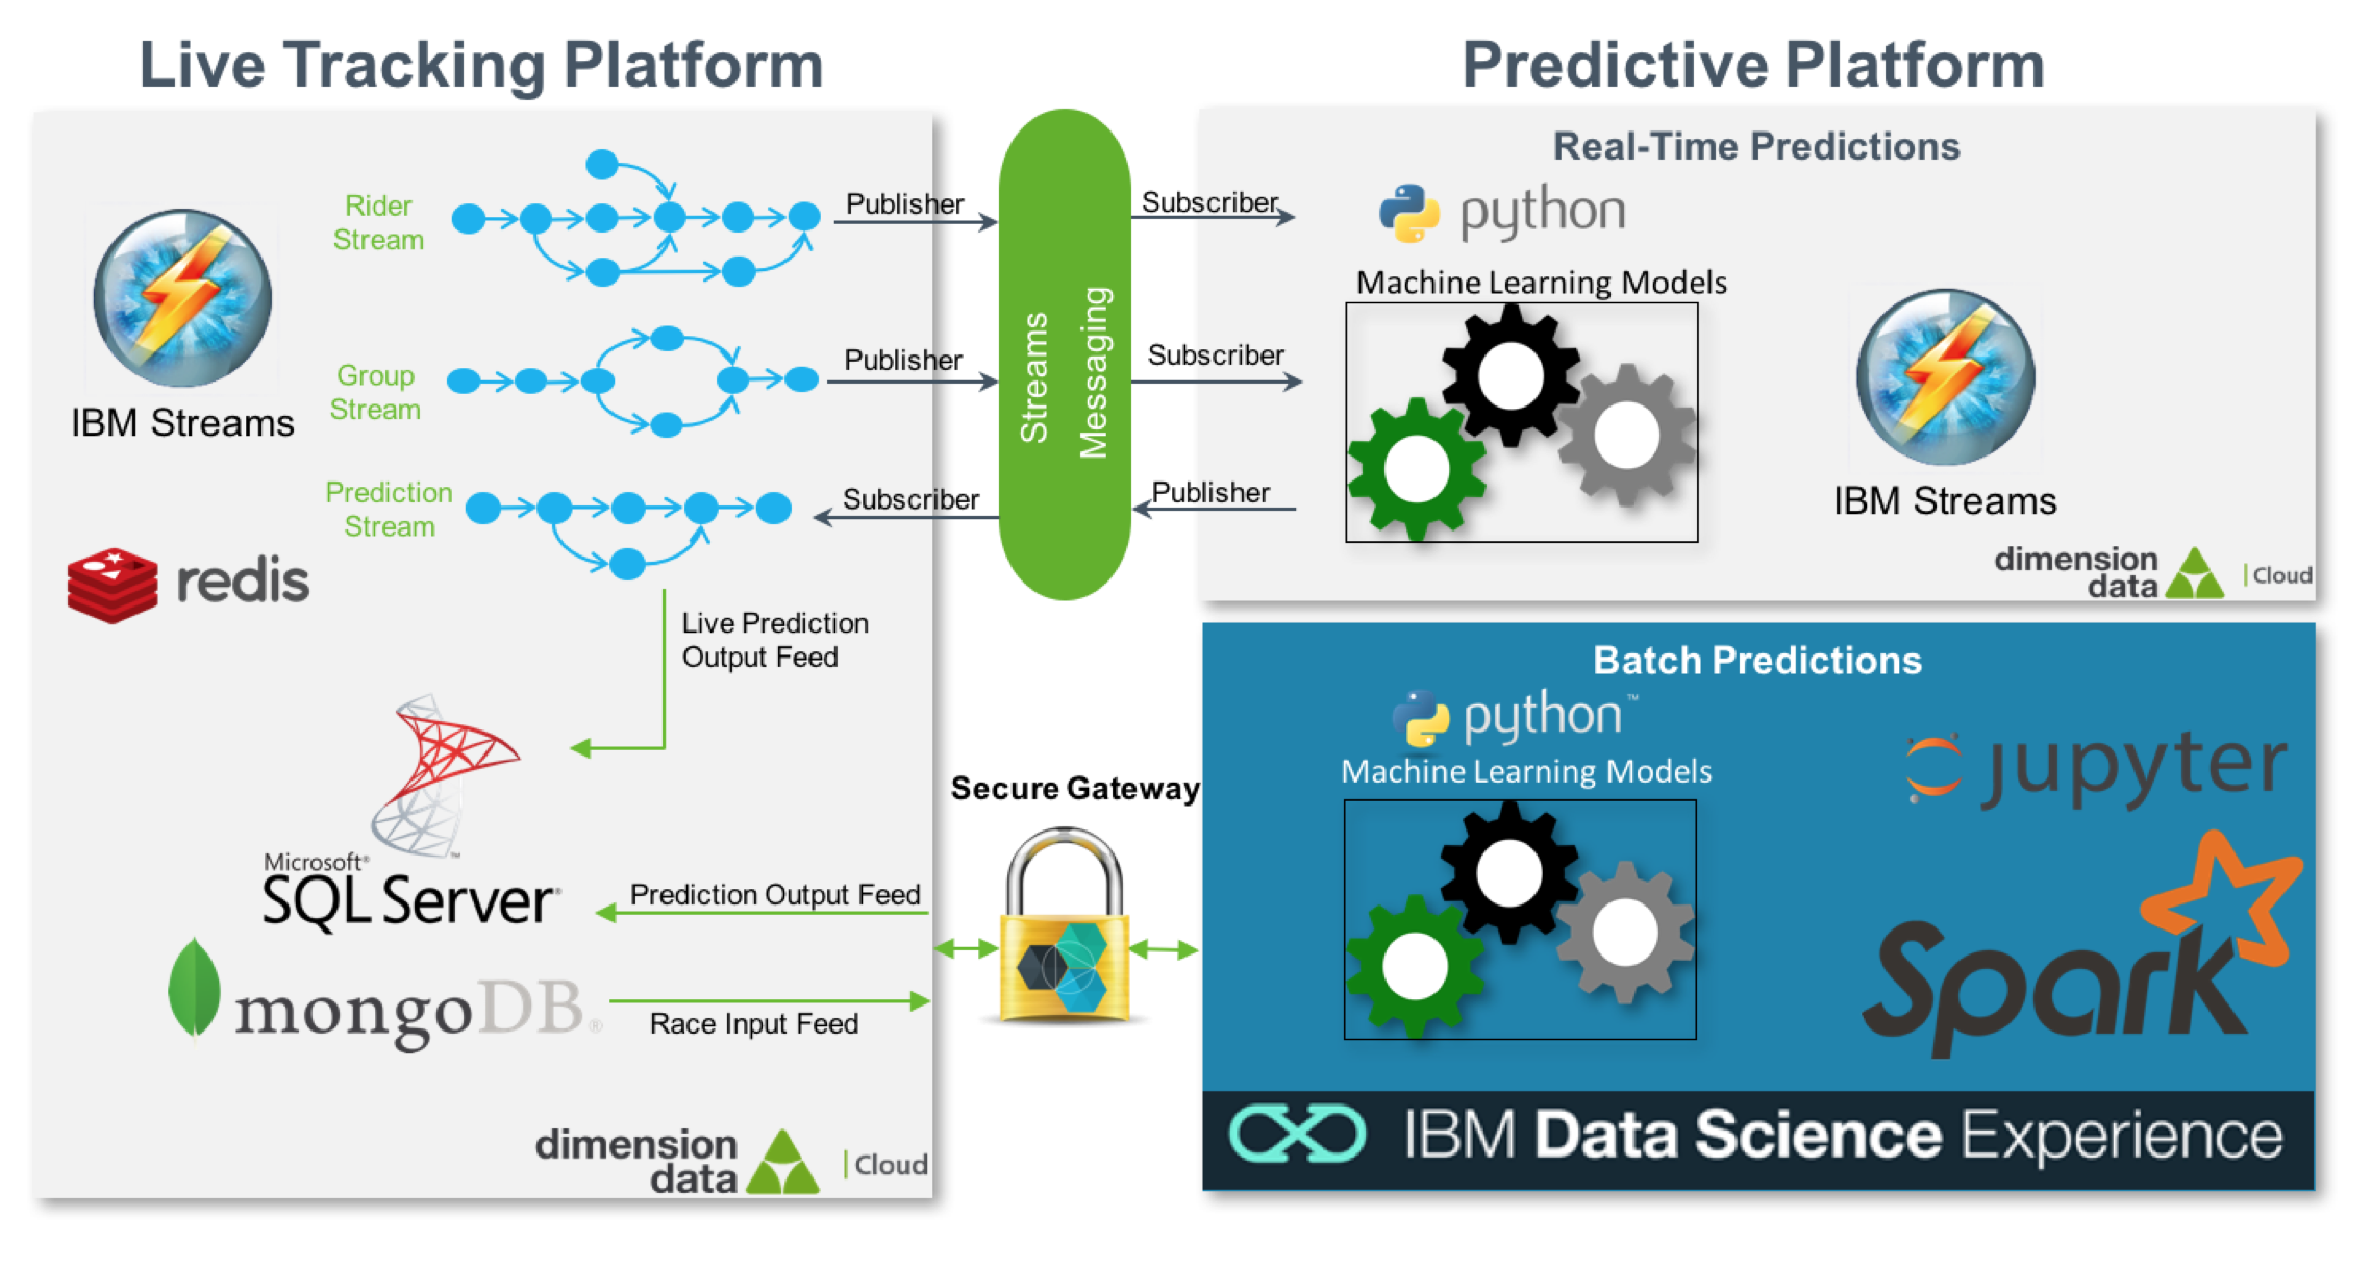
\includegraphics[width=\textwidth]{fig/TDF_system_architecture.eps}
 \caption{Real-time data streaming architecture of data collection
 platform that was used in {\it{Tour de France 2017}}}
 \label{fig:data_collection_platform}
\end{figure}

\end{document}

